\documentclass{article}


% load package with some of the available options - you may not need this!
\usepackage[framed,autolinebreaks,useliterate]{mcode}
% for checklist
\usepackage{enumitem,amssymb}
\newlist{todolist}{itemize}{2}
\setlist[todolist]{label=$\square$}
\usepackage{pifont}
\newcommand{\cmark}{\ding{51}}%
\newcommand{\xmark}{\ding{55}}%
\newcommand{\done}{\rlap{$\square$}{\raisebox{2pt}{\large\hspace{1pt}\cmark}}%
\hspace{-2.5pt}}
\newcommand{\wontfix}{\rlap{$\square$}{\large\hspace{1pt}\xmark}}


% something NOT relevant to the usage of the package.
\usepackage{graphicx}
\usepackage{url,textcomp}
\setlength{\parindent}{0pt}
\setlength{\parskip}{18pt}
\title{ECTA Homework 2\\Genetic Algorithms\\and\\TSP}
\author{\color{blue}Erick Kramer, Mihir Patil\\ \texttt{\color{blue}erick.romero@smail.inf.h-brs.de , mihir.patil@smail.inf.h-brs.de}}
% //////////////////////////////////////////////////

\begin{document}

\maketitle

\section{Assignment Description}
	\begin{enumerate}
		\item{Write a Genetic Algorithm to solve the Traveling Salesman Problem (TSP)}
		\begin{itemize}
			\item{All cities visited once, coming back to the start city}
			\item{100 largest cities in Germany (data files on LEA)}
			\item{Minimize the distance traveled}
		\end{itemize}
		\item{This time, to give you further insight into the inner workings of genetic algorithms we would like you to compare different mutation and crossover rates. Please use the plotting templates from the last weeks homework for your comparision. Use the parameters listed below for you comparision and explain the observed effects. Therefore please test and compare the effects of 4 different mutation rates and 4 different crossover rates.}
		\begin{itemize}
			\item{Mutation rates:}
			\item[-]{1/nCities\%}
			\item[-]{1\%}
			\item[-]{10\%}
			\item[-]{99\%}
			\item{Crossover rates:}
			\item[-]{1\%}
			\item[-]{10\%}
			\item[-]{80\%}
			\item[-]{99\%}
		\end{itemize}
		\item{Ensure a large enough sample for reliable results by repeating the experiments at least 30 times and reporting the median}
	\end{enumerate}


\section{The Assignment}

\subsection{Coding GA for TSP}
\begin{enumerate}
%-------------------------%
% Put your code here:

\item \textbf{Tournament Selection}
	\lstinputlisting[firstline=31, lastline=53]{my_selection_T.m}
	
\newpage

\item \textbf{Crossover}
	\lstinputlisting[firstline=33, lastline=80]{my_crossover_T.m}
	
\item \textbf{Mutation}
	\lstinputlisting[firstline=30, lastline=51]{my_mutation_T.m}
	
\item \textbf{Elitism}
	\lstinputlisting[firstline=26, lastline=38]{my_elitism_T.m}	
	
%-------------------------%
\end{enumerate}

\subsubsection{Comparing Algorithms}
\newpage

	\lstinputlisting[firstline=45, lastline=64]{code/monkeyExperiment.m}

	\begin{figure}[http]
	\begin{center}
	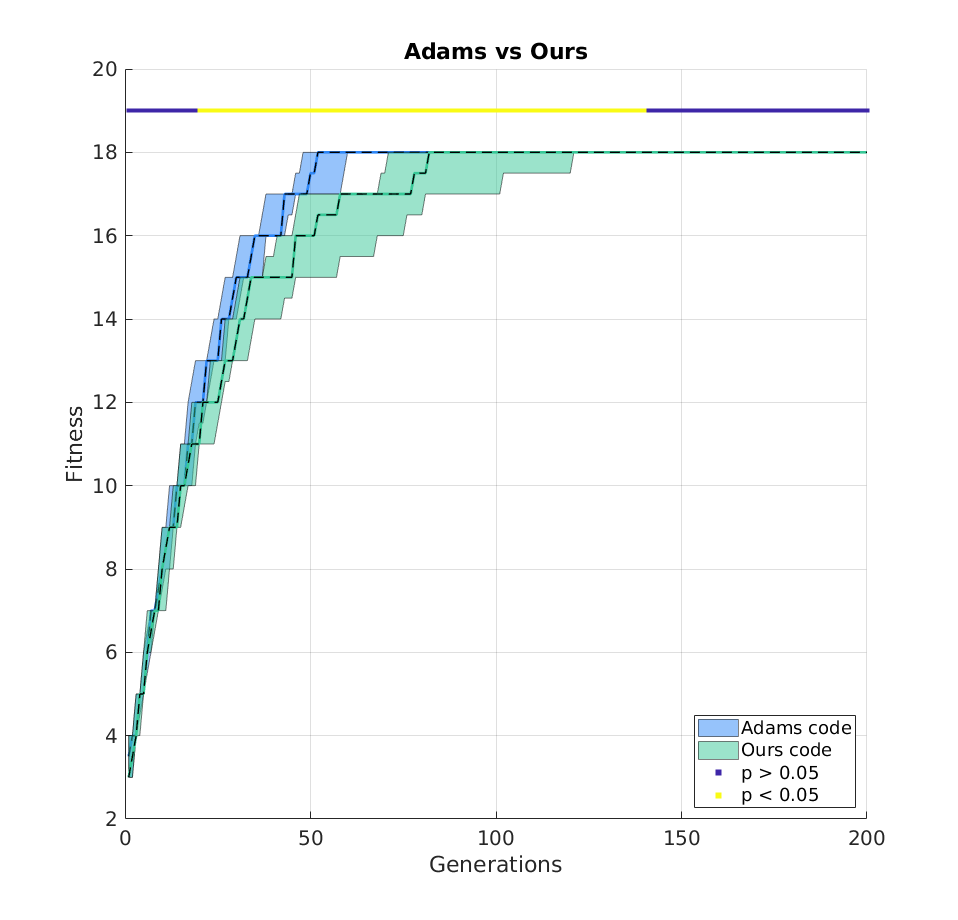
\includegraphics[scale=0.3]{img/Full_vsStandard.png}
	\caption{Graph comparing the performance of Adam's code vs ours.}
	\end{center}
	\end{figure}
	
	This plot shows the median performance at each generation (dashed lines) of each algorithm along with their upper and lower quartiles. Indicated at the top is the probability that the two algorithms are the same. Unsurprisingly, both runs of the same algorithm are statistically the same. Replace this plot with one of your own creation, comparing my code with your own implementation, to ensure that your code is working.
\newpage
	Perform the following comparisons of your algorithm with various components removed and replace the plots with your own, this can be done by replacing the functions in the code and saving the result (e.g. replacing the \mcode{my_crossover} function with the \mcode{no_crossover} function: (1) Your full implementation vs. No crossover, (2) Your full implementation vs. No mutation, (3) No crossover vs. No crossover AND no elitism, and (4) No mutation  vs. No mutation AND no elitism.

		\begin{figure}[h!]
		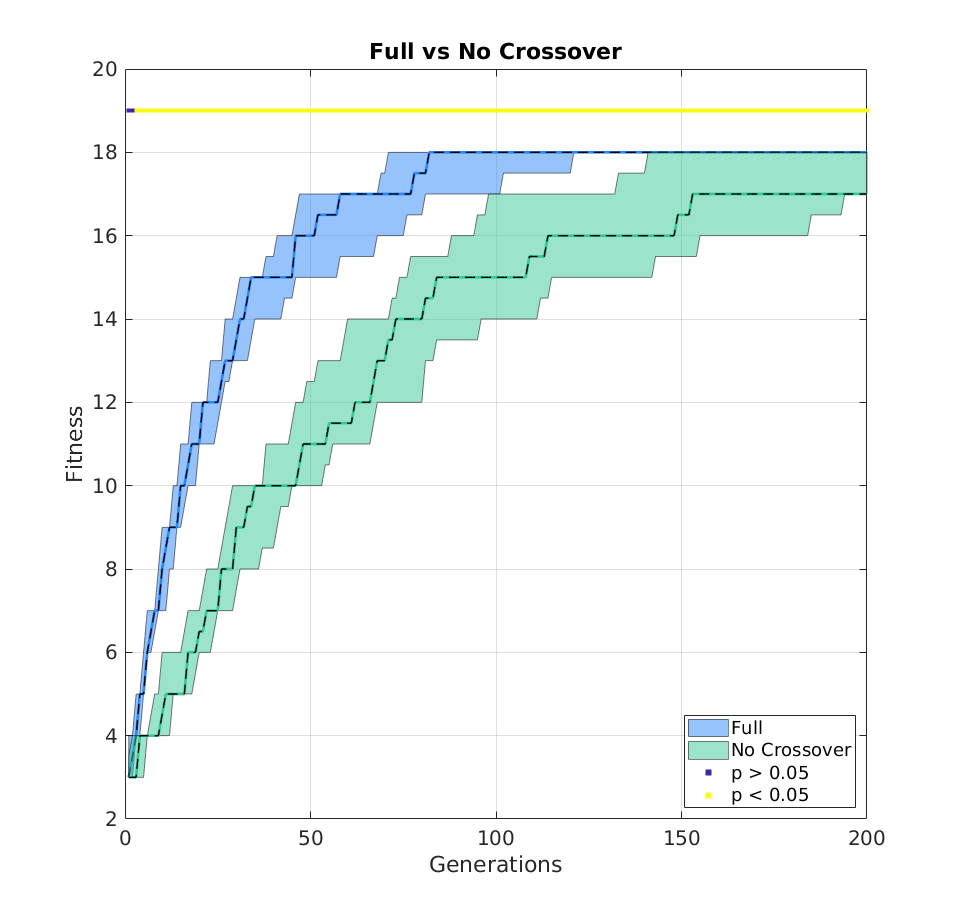
\includegraphics[width=0.5\textwidth]{img/Full_vsNoCross.png}
		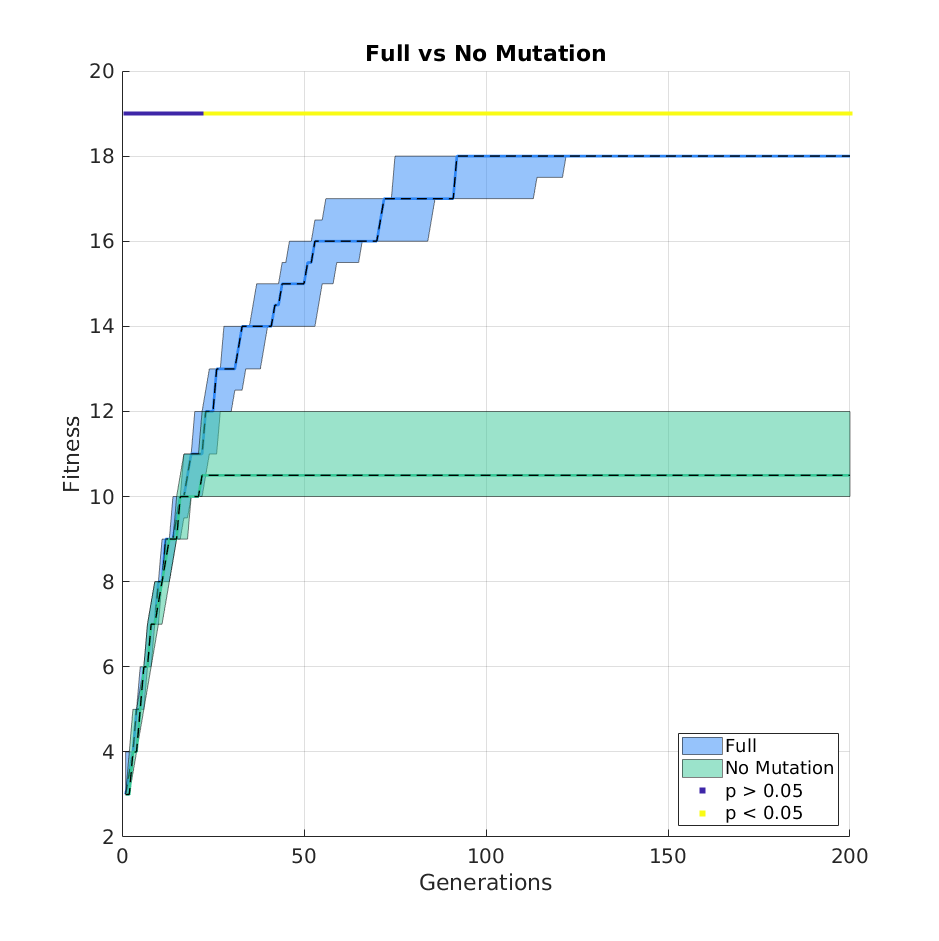
\includegraphics[width=0.5\textwidth]{img/Full_vsNoMut.png}
		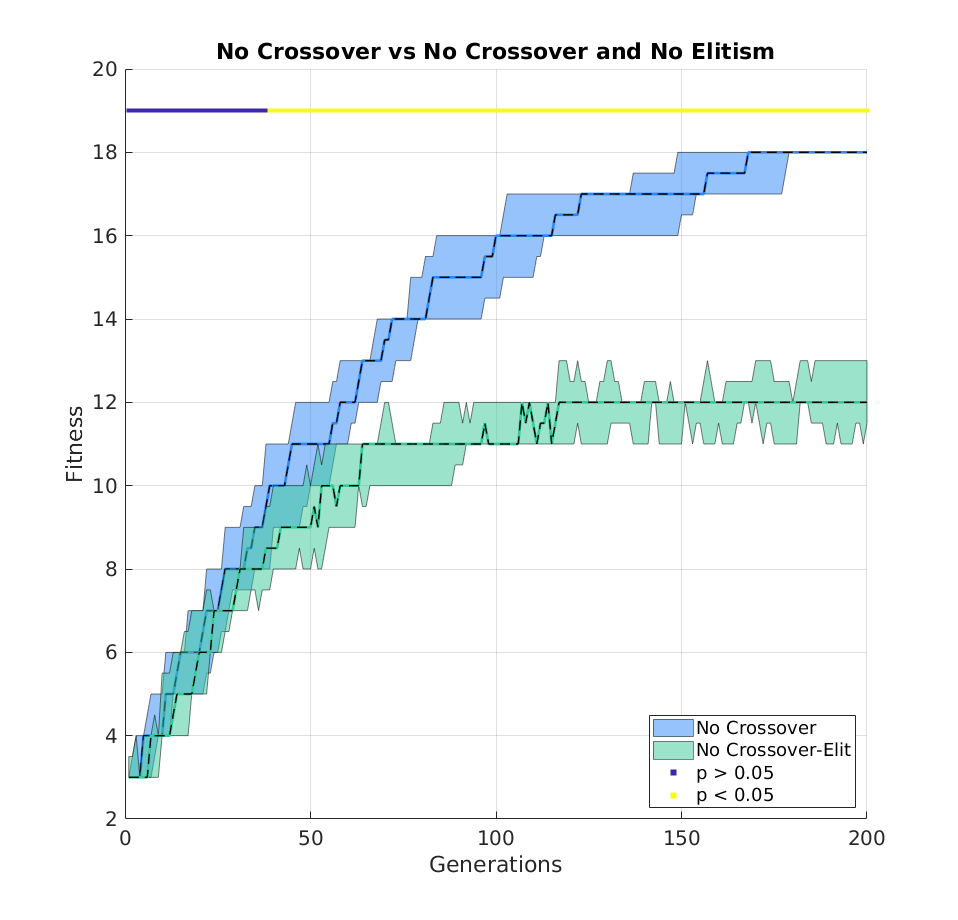
\includegraphics[width=0.5\textwidth]{img/NoCross_vsNoCrossNoElite.png}
		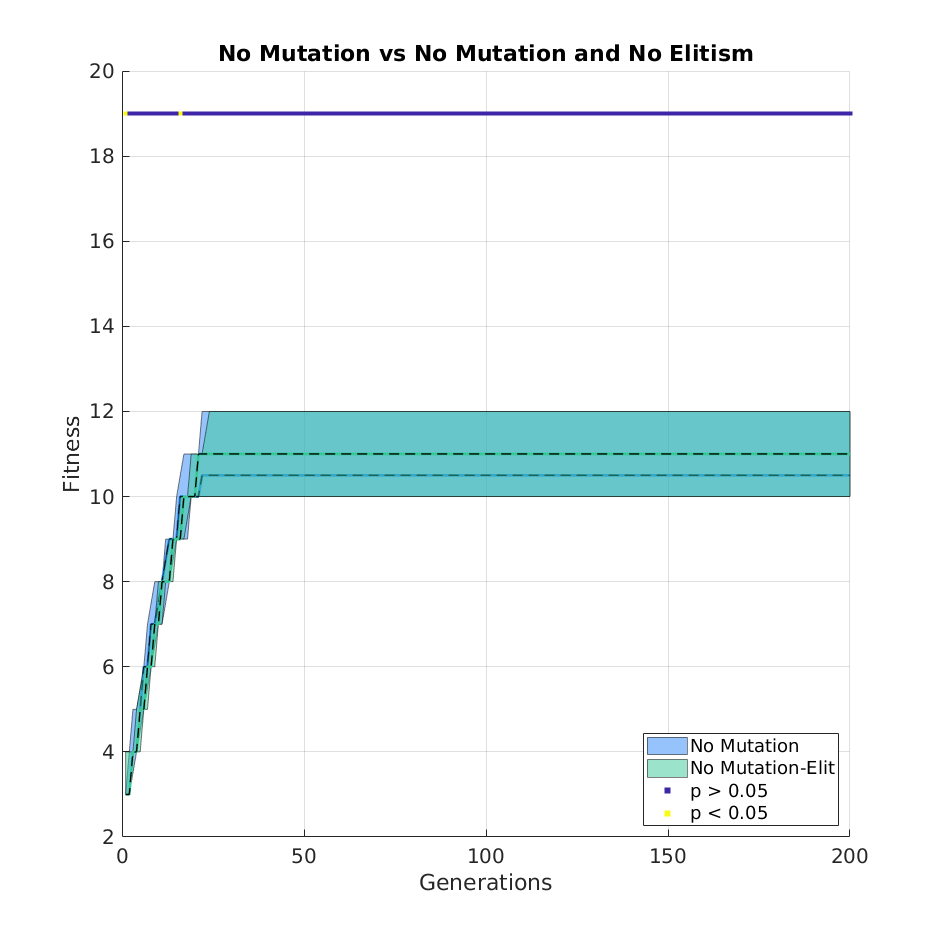
\includegraphics[width=0.5\textwidth]{img/NoMut_vsNoMutNoElite.png}
		\caption
		{
		\textbf{GA performance when operators are removed}\newline
		\textit{Top Left:} No Crossover,
		\textit{Top Right:} No Mutation, 
		\textit{Bottom Left:} No Crossover vs. No Crossover and No Elitism, 
		\textit{Bottom Right:} No Mutation and No Elitism
		}
		\end{figure}
\newpage
\subsubsection{Analyzing the Results}
\begin{enumerate}
	\item \textbf{Describe the main purposes of crossover and of mutation, how do your results illustrate their operation?} \\
%-------------------------%
% ANSWER: 
\textit{
 \color{blue}Crossover and mutation are techniques used ot add variability to the given population, while crossover works on the principle of recombination from two different parents mutation simply alters the value of a given gene in the chromosome. Also while crossover might lead to the convergence of the population to the local optima, mutation avoids the same problem by introducing new genetic material to the existing population.
 }
%-------------------------%

	\item \textbf{When only crossover is used the problem is not typically solved. Why? Could you devise an experiment that would support your explanation? One in which crossover could the solve the problem every time?}\\
%-------------------------%
% ANSWER:
\textit{
\color{blue}When only crossover is used the problem is not typically solved as the solution is derived from a bias existing genes. Hence other solutions aren't explored and the obtained solution may only be a single solution in a set of possible solutions. One possible experiment where crossover could always solve the problem would be the TSP problem.
 }
%-------------------------%
	
	\item \textbf{Describe the benefits of elitism in the crossover and mutation only cases.}\\
%-------------------------%
% ANSWER:
\textit{
\color{blue}In cases of crossover and mutation, elitism helps preserve the best possible solution to a problem. it preserves the best chromosome, if found, and hence drastically increases the performance of the  genetic algorithm.
}
%-------------------------%	

\end{enumerate}

\newpage
\subsection{Monkeys on a Typewriter}
\subsubsection{Using the GA}
Now time to test your algorithm on the entire soliloquy. Is it really better than just banging on a typewriter? Switch out the fitness function and give the whole speech a try. It might take a little time, you may have to increase the number of generations to get to 100\%, for this purpose don't worry about replicates:

\lstinputlisting[firstline=67, lastline=76]{code/monkeyExperiment.m}

By using the \mcode{tic} and \mcode{toc} commands we can time how long a program takes to execute. How long did it take your algorithm to find the whole speech?\\
%-------------------------%
% ANSWER:
\textit{
\color{blue} We got 99.5851\% correct in 39.0192 seconds.
}
%-------------------------%	

\newpage
\subsubsection{Brute force}
%How long would it take to find the same solution by a monkey on a type writer, i.e. by brute force? The average and worst case for a brute force algorithm can be easily calculated by counting the possible states. Let's be charitable and say this is a particularly clever monkey, who is systematic and never typing the same thing twice. Lets be even more charitable and say that this clever monkey also has a MATLAB license and has created a program to do the typing for him. How many possible states are there? How long will it take this MATLAB monkey to explore them all? Please show your work and use appropriate units for your answer.

(hint: to time a very fast piece of code, repeat in many times and take the average time, like this: )
\lstinputlisting[firstline=12, lastline=21]{code/monkey_vs_typewriter.m}


%-------------------------%
% ANSWER:
\textit{
\color{blue}The number of possible states is $28^{1446}$. A single evaluation takes $1.2763e-06$ seconds. Therefore, the algorithm would take all the possible states times a single evaluation, which basically is infinity, or a single run if we are super lucky. 
}
%-------------------------%

\vspace{2cm}
How comparable are these methods? Is random search comparable to evolutionary search?\\
%-------------------------%
\textit{
\color{blue}Although Random search and Evolutionary search both apply a degree of randomness in their approach, Evolutionary algorithm advances faster than a random algorithm as it does not start each new iteration from scratch, it has a memory of the best solution in the previous iteration and uses this to converge faster to a best possible solution. Genetic algorithms also incorporate the rejection of the least favorable genes in each generation, which is not possible with Random search.
}
%-------------------------%	






\newpage
\section{Inserting MATLAB code into LATEX --- 3 ways}

1) This inline demo \mcode{for i=1:3, disp('cool'); end;} uses the \verb|\mcode{}| command.\footnote{Works also in footnotes: \mcodefn{for i=1:3, disp('cool'); end;}}

2) The following is a block using the \verb|lstlisting| environment.
\begin{lstlisting}
for i = 1:3
	if i >= 5 && a ~= b       % literate programming replacement
		disp('cool');           % comment with some §\mcommentfont\LaTeX in it: $\mcommentfont\pi x^2$§
	end
	[:,ind] = max(vec);
	x_last = x(1,end) - 1;
	v(end);
	really really long really really long really really long really really long really really long line % blaaaaaaaa
	ylabel('Voltage (µV)');
end
\end{lstlisting}
Note: Here, the package was loaded with the \verb|framed|, \verb|numbered|, \verb|autolinebreaks| and \verb|useliterate| options.  \textbf{Please see the top of mcode.sty for a detailed explanation of these options.}


3) Finally, you can also directly include an external m-file from somewhere on your hard drive (the very code you use in \textsc{Matlab}, if you want) using the \verb|\lstinputlisting{/SOME/PATH/FILENAME.M}| command.  If you only want to include certain lines from that file (for instance to skip a header), you can use \verb|\lstinputlisting[firstline=6, lastline=15]{/SOME/PATH/FILENAME.M}|.


\end{document}